% Exposé III, first part: Definition III.1 to Proposition III.8.
% Sources: theory/framework.md (Exposé III, Def III.1 to Prop III.8), site/sections/06-fibres.html,
% theory/propositions.json (public statements of III.2 to III.8).
\section{Fibres and metrics: dynamics}\label{sec:fibres}

Expressivity lives on the image. Training lives on the fibres, through a metric. The image of a method fixes what it can reach, while its fibres and the optimizer's metric fix how it gets there. So two objects of $\Meth$ can be isomorphic and still train differently, and methods that look different can train identically.

Training happens upstairs, in the parameter space $Q$, where each fibre of $\rho$ collects the parameters that give one weight. The optimizer's metric on $Q$, pushed down to weight space, is what the model feels. Every statement below names its optimizer.

The exposé has four movements. Training with rates $\Lambda$ moves the weights by $\dot\theta=-K\nabla_\theta L$, with the cometric $K=D\rho\,\Lambda\,D\rho^\top$, which depends on where the parameters sit in their fibre (\thmref{Definition}{III.1} to \thmref{Proposition}{III.4}). Gradient flow conserves LoRA's charge $\Phi=B^\top B/\eta_B-AA^\top/\eta_A$, which sorts initialisations (\thmref{Theorem}{III.5} to \thmref{Proposition}{III.8}); when the charge is isotropic, one scale $\sigma^*$ separates a LoRA-FA-like regime from balanced dynamics (\thmref{Theorem}{III.9}). A 2-torus of rescalings acts on LoRA's knobs $(\alpha,\eta_A,\eta_B,\sigma_A)$ without changing training. Under Adam with $\varepsilon=0$, no decay or clipping and one shared schedule, LoRA+ with ratio $\lambda$ is plain LoRA with $\alpha$ multiplied by $\lambda$ (\thmref{Theorem}{III.10}, \thmref{Corollary}{III.11}, after \citealp{schulman2025lora}). Finally, SGD respects the subgroup $\Ort(r)$ of the gauge and Adam only the signed permutations. So from a zero-$B$ start the image depends only on $\operatorname{row}A_0$, the SGD trajectory on $A_0^\top A_0$, and the Adam trajectory on $A_0$ up to signed row permutations (\thmref{Theorem}{III.12}, \thmref{Corollary}{III.13}).

\subsubsection{One experiment first}\label{sec:fibres-hook}

Figure~\ref{fig:orbit} shows the cleanest consequence. Train with Adam at $\varepsilon=0$ from $B_0=0$, with no weight decay or clipping, one schedule for both parameter groups, and the same data order and dropout masks. Then LoRA+ with ratio $\lambda$ ($\eta_B=\lambda\eta_A$) and plain LoRA with $\alpha$ multiplied by $\lambda$, at the same $\eta_A$ and $A_0$, produce the same weights at every step (\thmref{Theorem}{III.10}, \thmref{Corollary}{III.11}). This LoRA/Adam statement is due to \citet{schulman2025lora}, for the LoRA+ of \citet{hayou2024lora}; \thmref{Theorem}{III.10} says what is added here.

\subsubsection{The metric a method carries}\label{sec:fibres-cometric}

A learning rate is a metric in disguise. Gradient descent with rates $\Lambda$ moves $q$ by $-\Lambda\nabla_q$, and pushed down by $D\rho$ this is the weight gradient multiplied by a positive semidefinite operator.

\begin{definition}{III.1}{trained method; cometric; three equivalences}
A \emph{trained method} is a method together with optimizer data: a learning-rate operator $\Lambda\succ0$ (per-block rates), an initial scale, and an update rule. Gradient flow $\dot q=-\Lambda\nabla_q(L\circ\rho)$ moves the weights by
\[\dot\theta=-K_q\nabla_\theta L,\qquad K_q=D\rho_q\,\Lambda\,D\rho_q^\top.\]
We call $K_q$ the \textbf{induced cometric}. For a backward method with compression $c_t$ and anchor $a_t$ (\thmref{Definition}{IV.1}), $K_t=a_tc_t$.

Two methods are
\begin{itemize}
\item \emph{expressively equivalent} if their images agree;
\item \emph{first-order equivalent} if their $K_{q_0}$ agree;
\item \emph{dynamically equivalent} if they produce the same $\theta$-trajectory for every loss.
\end{itemize}
\end{definition}

Cometrics compose the way derivatives do.

\begin{observation}{III.2}{chain rule for cometrics}
Let $\sigma:Q'\to Q$ and $\rho:Q\to X$ be smooth, with $X=\Theta$ or a function or output space. Train $Q'$ by gradient flow with a constant rate operator $\Lambda'\succ0$, and put $K^\sigma_{q'}:=D\sigma_{q'}\Lambda'D\sigma_{q'}^\top$. Then
\[K^{\rho\sigma}_{q'}=D\rho_{\sigma(q')}\,K^\sigma_{q'}\,D\rho_{\sigma(q')}^\top,\]
and no metric on $Q$ is used. $K$ is a degenerate cometric (positive semidefinite, of rank $\le\dim Q'$); when $\sigma$ is not injective, $K^\sigma$ is a field along $\sigma$ and fails to be a cometric on $Q$.

For LoRA \citep{hu2021lora}, $\rho(B,A)=W_0+sBA$ with $s=\alpha/r$ ($\alpha/\sqrt r$ for rsLoRA, \citealp{kalajdzievski2023rank}), block rates $\Lambda=\diag(\eta_BI,\eta_AI)$ and no LoRA dropout, under gradient flow (equivalently, to first order in the step size for GD),
\[K_{(B,A)}(G)=s^2\big(\eta_B\,GA^\top A+\eta_A\,BB^\top G\big).\]
Under Adam there is no state-independent linear cometric; \thmref{Theorem}{III.10} and \thmref{Theorem}{III.12} treat Adam.
\end{observation}

\noindent\labelsf{Num}\enspace Finite-difference Jacobians agree with the formula to $6\times10^{-9}$ (Appendix~\ref{app:repro}).

\begin{explains}
For LoRA, the term $\eta_B\,GA^\top A$ lets the update reach all outputs while filtering its inputs through $\operatorname{row}A$, and $\eta_A\,BB^\top G$ does the reverse. At $B_0=0$ only the first term survives, so the first-step cometric $s^2\eta_B\,GA_0^\top A_0$ is fixed by $A_0$ (\thmref{Corollary}{III.13}).

\smallskip
Take $X$ to be the prefix space (Exposé~\ref{sec:merge}). HF \texttt{PrefixTuning} with \texttt{prefix\_projection=True} (the MLP $\sigma$ of \citealp{li2021prefix}) and with \texttt{prefix\_projection=False} (the P-tuning v2 setting of \citealp{liu2021p}, ignoring its classification head) have the same prefix image whenever \texttt{encoder\_hidden\_size}${}\ge{}$\texttt{num\_virtual\_tokens}${}-1$. Under gradient flow their cometrics on prefix space are $D\sigma\Lambda'D\sigma^\top$ and $\Lambda$, so the reparametrisation replaces the flat metric on prefix space by a point-dependent one. Prefix methods are extensions, so the target here is the prefix (or function) space rather than $\Theta$. This alone does not account for the instability that Li and Liang observed under AdamW.
\end{explains}

Backpropagation as a lens, the source of this chain rule, is due to \citet{fong2017backprop} and \citet{cruttwell2021categorical}.

\subsubsection{When a change of chart does not matter}\label{sec:fibres-naturality}

A gauge transformation changes the parameters and keeps the weights. It leaves training unchanged exactly when the cometrics agree, which for LoRA's gauge $\GL_r$ singles out $\Ort(r)$.

\begin{theorem}{III.3}{gradient descent is natural exactly where cometrics agree; for LoRA's linear gauge, exactly along $\Ort(r)$}
(a) Let $\varphi:Q\to Q'$ be a diffeomorphism with $\rho'\circ\varphi=\rho$, and let $\Lambda,\Lambda'$ be the rate operators on $Q,Q'$. Under gradient flow, the two methods induce the same $\theta$-velocity at $q$ and at $\varphi(q)$ for every loss iff $K^\rho_q=K^{\rho'}_{\varphi(q)}$, that is,
\[D\rho'_{\varphi(q)}\big(D\varphi_q\Lambda D\varphi_q^\top-\Lambda'\big)D\rho'^\top_{\varphi(q)}=0.\]
This holds whenever $D\varphi\Lambda D\varphi^\top=\Lambda'$, which is an isometry when $\Lambda=\Lambda'=I$. That condition is necessary when $D\rho'_{\varphi(q)}$ is injective, and fails to be necessary in general. Every linear gauge of a linear parametrisation is natural; for instance, for $\rho(x,y)=\theta_0+x+y$ the shear $(x,y)\mapsto(2x,y-x)$ preserves $\rho$ and $K$ without being orthogonal. So is every pointwise-orthogonal non-linear LoRA gauge $\varphi(q)=\varphi_{g(q)}(q)$ with $g(q)\in\Ort(r)$.

(b) For LoRA's linear gauge $\varphi_g(B,A)=(Bg^{-1},gA)$ with block-scalar rates, at points where $A$ has full row rank ($B$ arbitrary, including $B=0$) and $r<n$, the criterion holds iff $g\in\Ort(r)$. The same holds symmetrically where $B$ has full column rank and $r<m$.
\end{theorem}

\noindent\labelsf{Num}\enspace At a random point a non-orthogonal $g$ gives a cometric mismatch of about $18$, an orthogonal one about $10^{-15}$ (Appendix~\ref{app:repro}).

\begin{explains}
No learner with a fixed Euclidean metric respects all invertible reparametrisations. For LoRA's linear gauge, plain gradient descent defines a family of training dynamics indexed by the cosets $\Ort(r)\backslash\GL_r$, which $g\mapsto g^\top g$ identifies with $\Sym^+_r$. Under gradient descent, LoRA+'s rate ratio $\lambda$ corresponds to the scalar gauge $g=\lambda^{1/4}I$ together with an overall change of rate. rsLoRA rescales $s$, equivalently the learning rates and the initialisation; this is a move on the hyperparameter torus and involves no choice of gauge (\thmref{Theorem}{III.10}, \thmref{Corollary}{III.11}). Riemannian preconditioning and LoRA-Pro remove the dependence on the representative (\thmref{Proposition}{III.4}). Under AdamW, as used in practice, the relevant group is the group $B_r$ of signed permutations (\thmref{Theorem}{III.12}).
\end{explains}

The $\GL_r$ symmetry of $W=BA$ and the quotient geometry of fixed-rank matrices are classical \citep{mishra2012fixed}. \citet{putterman2024learning} build learners on LoRA weights that respect it.

Some published optimizers use instead a cometric that depends only on the weight, at least in an idealised form.

\begin{proposition}{III.4}{cometrics that descend to the rank-$r$ manifold; known in part}
Write $U=\operatorname{col}B$ and $V=\operatorname{row}A$. Statements (a), (b) and the first sentence of (d) are on the full-rank locus; (c) needs only $\rk A_0=r$, with $B$ arbitrary, including $B_0=0$. All statements concern gradient flow, or (S)GD to first order, on the stated gradients, undamped and without Adam. Cometrics include the learning rate.

(a) Scaled GD, $\delta B=-\eta\nabla_B(AA^\top)^{-1}$ and $\delta A=-\eta(B^\top B)^{-1}\nabla_A$, is $\GL_r$-equivariant with first-order cometric $K(G)=\eta s^2(P_UG+GP_V)$.

(b) LoRA-Pro's equivalent gradient $\tilde g=P_UG+(I-P_U)GP_V$ is the Frobenius-orthogonal projection $\Pi_{T_{W-W_0}\MM_r}(G)$. The flow of its SGD variant (LoRA-Pro Alg.~1) is the Riemannian gradient flow (\bgref{D.24}) on $W_0+\MM_r$.

(c) LoRA-FA's corrected gradient $s^{-2}\nabla_B(A_0A_0^\top)^{-1}$, fed to SGD with $A_0$ frozen, gives $K(G)=\eta\,GP_V$ with $V=\operatorname{row}A_0$, which depends on $A_0$ only through $V\in\Gr(r,n)$. Its original form, plain SGD on $B$, has $K(G)=s^2\eta_BGA_0^\top A_0$.

(d) The cometrics of (a) and (b) are functions of $W$ on the full-rank locus and define vector fields tangent to $W_0+\MM_r$. The field of (c) is $G\mapsto\eta GP_V$ with $V=\operatorname{row}A_0$. Its flow is the Frobenius gradient flow on the slice $W_0+\{XA_0\}=W_0+\R^{m\times n}P_V$, of dimension $mr$, which contains $W_0$ and lies in $W_0+\Mr$. The rank-$r$ part of the slice, $N_V=\{\operatorname{row}(W-W_0)=V\}$, is open and dense in it and is a submanifold of $W_0+\MM_r$. On $N_V$ the field is tangent to $\MM_r$ and equals $\eta GP_{\operatorname{row}(W-W_0)}$, a function of $W$. So (c) descends too, as a degenerate cometric of rank $mr$ (less than $r(m+n-r)$ when $r<n$) whose flow keeps $\operatorname{row}(W-W_0)=\operatorname{row}A_0$ fixed. The cometric of plain GD depends on the representative; it is invariant only under $\Ort(r)$.
\end{proposition}

The algorithms are known. Scaled GD is due to \citet{xtong2021accelerating} and \citet{zhang2024riemannian}, and LoRA-Pro to \citet{wang2024lorac}. LoRA-FA in its frozen-$A$ form is \citet{zhang2023lora}; the corrected gradient of (c) comes from the 2026 revisions (v2 and v3) of that arXiv record and from the LoRA-FA optimizer added to HF PEFT \citep{xmangrulkar2022peft} in 2025. The $\GL_r$-invariance of the scaled-GD metric and its descent to the quotient $\MM_r$ are classical \citep{mishra2012fixed,xmishra2016riemannian}.

\noindent\labelsf{Num}\enspace Gauge defects are about $10^{-15}$ for (a), against $52$ for plain GD. LoRA-FA with AdamW from $A_0$ and from $gA_0$ differs by $O(1)$ after a few steps, against $10^{-15}$ with SGD (Appendix~\ref{app:repro}).

\paragraph{Practice} Each published method departs from these idealisations, and the departures change the symmetry (\thmref{Theorem}{III.12}).
\begin{itemize}
\item The standard start $B_0=0$ lies off the full-rank locus, where (a) and (b) are undefined without damping. \citet{zhang2024riemannian} use $(B^\top B+\delta I)^{-1}$ with an unspecified $\delta>0$, which is only $\Ort(r)$-equivariant. Their LLM experiments report both damped scaled GD and scaled AdamW, in which the preconditioner is applied before the Adam moments ($B_r$). HF's \texttt{create\_riemannian\_optimizer} damps as well.
\item LoRA-Pro's experiments use its AdamW variant (Alg.~2, with $m\times n$ moments), $\dot W=-\Pi_T(\mathrm{Adam}(\Pi_TG))$. It descends to $W_0+\MM_r$ without being a gradient flow, and its discrete update with the Sylvester-optimal free matrix (\bgref{D.33}) is $\GL_r$-invariant only to first order. The released code also damps both inverses ($\operatorname{pinv}(\cdot+10^{-8}I)$, so $\Ort(r)$), replaces the step at $B_0=0$ by a LoRA-FA-type step, and runs with HF's default global-norm clipping.
\item LoRA-FA as published (v3, Alg.~1) and HF's \texttt{create\_lorafa\_optimizer} apply AdamW after the correction (HF also damps with $10^{-8}I$). The trajectory is then invariant only under signed row permutations of $A_0$ (\thmref{Theorem}{III.12}(b)), so it depends on the basis and scale of $A_0$ as well as on $\operatorname{row}A_0$.
\end{itemize}

\begin{remark*}{2026: Riemannion}
Riemannion \citep{bogachev2025lora} defines its optimizer on $\MM_r$ directly. Its variable is the point $X\in\MM_r$, stored as thin factors, and apart from weight decay each step uses only $X$, the projected gradient and the momentum: the tangent projection of \thmref{Proposition}{III.4}(b), momentum carried along by the same projection, a Muon step \citep{xjordan2024muon} that sets the nonzero singular values of the momentum to $1$ and projects again, and a truncated SVD as retraction. No Gram matrix is inverted, so nothing needs damping, and with weight decay off, the $W$-trajectory, momentum included, does not depend on how $X$ is factored. The published Algorithm~4 writes its weight decay through the orthonormal factors, as a term $\gamma A_LB_R^\top$, so this holds for $\gamma=0$. Its non-linearity acts on a weight-space matrix, while Adam's acts coordinatewise on the factors, which is what cuts the gauge down to $B_r$ (\thmref{Theorem}{III.12}).
\end{remark*}

\begin{explains}
Under (S)GD each method is summarised by its induced weight-space cometric (Table~\ref{tab:cometrics}). LoRA, scaled GD and LoRA-Pro share the image $W_0+\Mr$ and differ only in cometric. LoRA-FA is the sub-object $W_0+\{XA_0\}$ (\thmref{Corollary}{III.13}). GaLore (with a gradient-SVD or a random projector) and MeZO are full-parameter methods, listed for comparison. Flora proper compresses only its momentum, takes full-space Adafactor steps, and has no cometric of this form (Exposé~\ref{sec:lens}).
\end{explains}

\begin{table}[t]
\centering\small\renewcommand{\arraystretch}{1.12}
\caption{Induced weight-space cometrics under gradient flow or SGD (\thmref{Observation}{III.2}, \thmref{Proposition}{III.4}). The last three rows are full-parameter methods, listed for comparison; $P$ and $Q$ are GaLore's left and right projectors, $A_t$ a random projector, $z$ the random direction of MeZO.}\label{tab:cometrics}
\begin{tabularx}{\linewidth}{@{}>{\raggedright\arraybackslash}p{0.47\linewidth}>{\raggedright\arraybackslash}X@{}}
\toprule\headrow
\textbf{Method (gradient flow or SGD)} & \textbf{Cometric $K(G)$}\\
\midrule
LoRA \citep{hu2021lora} & $s^2(\eta_BGA^\top A+\eta_ABB^\top G)$\\
LoRA-FA, original / corrected \citep{zhang2023lora} & $s^2\eta_BGA_0^\top A_0$ / $\eta GP_V$\\
scaled GD, undamped Riemannian preconditioning \citep{xtong2021accelerating,zhang2024riemannian} & $\eta s^2(P_UG+GP_V)$\\
LoRA-Pro, SGD variant \citep{wang2024lorac} & $\eta\,\Pi_{T\MM_r}G$\\
GaLore, one period, scale $\alpha$ \citep{zhao2024galore}; \thmref{Proposition}{IV.2} & $\eta\alpha PP^\top G$, or $\eta\alpha\,GQQ^\top$ when $m>n$ (default $\alpha=0.25$)\\
GaLore with a random projector $A_t$, one period (the compressed SGD of \citealp{hao2024flora}) & $\eta GA_t^\top A_t$\\
MeZO \citep{malladi2023fine} & $\eta zz^\top G$, equal to $\eta G$ in expectation\\
\bottomrule
\end{tabularx}
\end{table}

``Transformation invariance'' in the sense of Definition~1 of LoRA-RITE \citep{yen2024lora} means that the $W$-update is invariant under the gauge ($W$-level descent), which is weaker than parameter-level $\GL_r$-equivariance. LoRA-RITE's algorithm satisfies the stronger property on the full-rank locus (\thmref{Theorem}{III.12}).

\subsubsection{Isometries and charges}\label{sec:fibres-charges}

Split LoRA's gauge in two. With per-block scalar rates, the antisymmetric generators rotate the rank channels and preserve the rate metric, so the optimizer cannot feel them. Along the symmetric ones, gradient flow conserves a quadratic charge (\bgref{D.26}). For LoRA the charges form one matrix $\Phi$, whose vanishing is the balancedness of deep linear networks (\bgref{D.28}).

\begin{theorem}{III.5}{Noether charges and isometries for cotangent signals; known, \citet{zhao2022symmetries}}
Let a Lie group act linearly on $Q=\R^N$ with $\rho\circ k=\rho$, let $\Lambda\succ0$ be constant, and let $\gamma(t)\in T^*_{\rho(q(t))}\Theta$ be any cotangent signal, gradient or not. Consider the continuous-time updates
\[\dot q=-\Lambda\,D\rho_q^\top\gamma(t).\]

(i) For every generator $\xi$ with $\Lambda^{-1}\xi$ symmetric, the charge $J_\xi(q)=\tfrac12\langle q,\Lambda^{-1}\xi q\rangle$ is conserved.

(ii) For every generator $\xi$ with $\Lambda^{-1}\xi$ antisymmetric, $k=e^{\tau\xi}$ preserves $\langle\cdot,\Lambda^{-1}\cdot\rangle$, so $K_{kq}=K_q$ along the orbit; for the same cotangent $\gamma$, the $\theta$-velocities at $q$ and at $kq$ agree. Suppose moreover that $\gamma$ depends on $q$ only through $(t,\rho(q))$, as $\gamma=\nabla_\theta L$ or an open-loop signal does, and that solutions are unique ($\gamma$ measurable in $t$ and locally Lipschitz in $\theta$, $\rho$ of class $C^{1,1}_{\mathrm{loc}}$). Then the $\theta$-trajectories from $q_0$ and from $kq_0$ coincide. If $\gamma$ uses Euclidean norms on $Q$, as global-norm clipping does, the trajectory statement holds when, in addition, $k$ is a Euclidean isometry, and can fail otherwise. So (i) and the velocity statement of (ii) hold for arbitrary $\gamma$, while the trajectory statement needs a gradient-like signal.

(iii) When $\mathfrak g$ is closed under $\xi\mapsto\Lambda\xi^\top\Lambda^{-1}$, every generator splits into a part of type (i) and a part of type (ii), a Cartan decomposition $\mathfrak g=\mathfrak k\oplus\mathfrak p$ (\bgref{D.27}). This holds for LoRA's $\gl_r$ with per-block scalar rates. Without closure, there are generators of neither type. With per-rank-channel rates $\Lambda(B,A)=(BD_B,D_AA)$, where $D_B=\diag(\eta_{B,j})$ and $D_A=\diag(\eta_{A,j})$, the generator $\xi_X$ is of type (i) iff $XD_B^{-1}$ and $D_A^{-1}X$ are both symmetric, and of type (ii) iff both are antisymmetric. An off-diagonal pair $(i,j)$ contributes one charge and one isometry iff $\eta_{B,i}\eta_{A,i}=\eta_{B,j}\eta_{A,j}$, and $\mathfrak g$ is closed iff all the products $\eta_{B,j}\eta_{A,j}$ are equal. In that case one gets a $D$-conjugate of $\so_r\oplus\Sym_r$ whose isometries are not all Euclidean unless the rates are
block-scalar, so the clipping caveat of (ii) applies. For pairwise distinct products, only the diagonal $X$ give charges and no nonzero $X$ gives an isometry.
\end{theorem}

Part (i) is \citet{zhao2022symmetries}, Prop.~5.1, including the table of symmetric and antisymmetric generators and symmetric learning rates. Laws that hold for every loss and dataset are characterised by \citet{marcotte2023abide}, and the principle goes back to \citet{du2018algorithmic}, \citet{arora2018optimization} and \citet{kunin2020neural}. New here are only the remark that $\gamma$ need not be a gradient, which is formally immediate (along the realised trajectory, $\gamma(t)$ is the gradient of the time-dependent linear loss $\langle\gamma(t),\theta\rangle$), and the PEFT instances below.

\noindent\labelsf{Num}\enspace With a non-gradient, $q$-dependent $\gamma$ on LoRA, $\Phi$ drifts by $1.6\times10^{-12}$. With Euclidean clipping and a non-Euclidean isometry $k$, the $\theta$-trajectories from $q_0$ and $kq_0$ differ by $0.06$. With per-channel rates $\eta_B=(1,1,1)$ and $\eta_A=(1,1,2)$ at $r=3$, closure fails, but $X=E_{12}+E_{21}$ still gives a conserved charge (Appendix~\ref{app:repro}).

\paragraph{Instances} All instances assume gradient flow, or SGD without momentum, with per-block rates. AdamW and heavy-ball momentum fall outside the theorem, since their buffers store $D\rho$ at past points.
\begin{itemize}
\item \textbf{LoRA.} The generators $\xi_X(B,A)=(BX,-XA)$ with $\Lambda=\diag(\eta_B,\eta_A)$ satisfy: $\Lambda^{-1}\xi_X$ is symmetric iff $X=X^\top$. So the $r(r+1)/2$ charges are the entries of
\[\Phi=\frac{B^\top B}{\eta_B}-\frac{AA^\top}{\eta_A},\]
which is ``balancedness'', the $\mathfrak p=\Sym_r$ half of $\gl_r=\so_r\oplus\Sym_r$. The $\so_r$ generators act by Euclidean isometries, so (ii) holds for LoRA even under global-norm clipping.
\item \textbf{DyLoRA} \citep{valipour2022dylora}. The gauge reduces to the torus, so only $\diag\Phi$ is conserved.
\item \textbf{VeRA} \citep{kopiczko2023vera}. The gauge is $(b,d)\mapsto(cb,d/c)$, with charge $\|b\|^2/\eta_b-\|d\|^2/\eta_d$. NOLA \citep{koohpayegani2023nola} is analogous.
\item \textbf{AdaLoRA} \citep{zhang2023adalora} ($P\Lambda Q$), without its orthogonality regulariser and between rank-budget masking events. Each torus edge gives a charge, $\|p_k\|^2-\lambda_k^2$ and $\|q_k\|^2-\lambda_k^2$, at equal rates. The regularised objective (HF default \texttt{orth\_reg\_weight=0.5}) breaks these charges.
\item \textbf{HRA} \citep{yuan2024bridging}. The rescaling $u_i\mapsto cu_i$ gives a conserved $\|u_i\|^2$.
\item \textbf{ReLU bottleneck adapters} \citep{houlsby2019parameter}. Positive per-unit rescalings give one charge per hidden unit.
\item \textbf{TT adapters} (for instance \citealp{yang2024loretta,anjum2024tensor}). One conserved matrix per bond.
\item \textbf{DoRA's detached-norm backward \citep{liu2024dora} and global-norm gradient clipping.} Both still have the form $\Lambda D\rho_{\mathrm{LoRA}}^\top\gamma$, with $\gamma$ the detached or clipped signal, so $\Phi$ is still conserved.
\end{itemize}

Under discrete GD with rates $\eta_B,\eta_A$, one step changes $\Phi$ by exactly
\[\eta_B\,AG^\top GA^\top-\eta_A\,B^\top GG^\top B,\]
so the drift of $\eta\Phi$, or the drift relative to $\Phi$, is $O(\eta^2)$ per step. Adam is not of the form $\Lambda D\rho^\top\gamma$, so the drift of $\Phi$ under Adam measures how far Adam departs from the gauge geometry; this is a prediction (Exposé~\ref{sec:predictions}).

\begin{explains}
Conservation needs only the shape $\dot q=-\Lambda D\rho^\top\gamma$, so it holds for any loss and any data. With $\eta$ the common scale of the rates, a GD step changes $\eta\Phi$ by $O(\eta^2)$ and an Adam step by $O(\eta)$, as panel (a) of Figure~\ref{fig:noether} shows.
\end{explains}

\begingroup\renewcommand{\label}[1]{}%
\begin{analogy*}{Noether; gauge}
\emph{Noether} names the passage from a symmetry to a conserved quantity, here proved for gradient flow without a Lagrangian. \emph{Gauge} means the symmetry group of a parametrisation; no connection is involved.
\end{analogy*}
\endgroup

\begin{figure}[tbp]
\centering
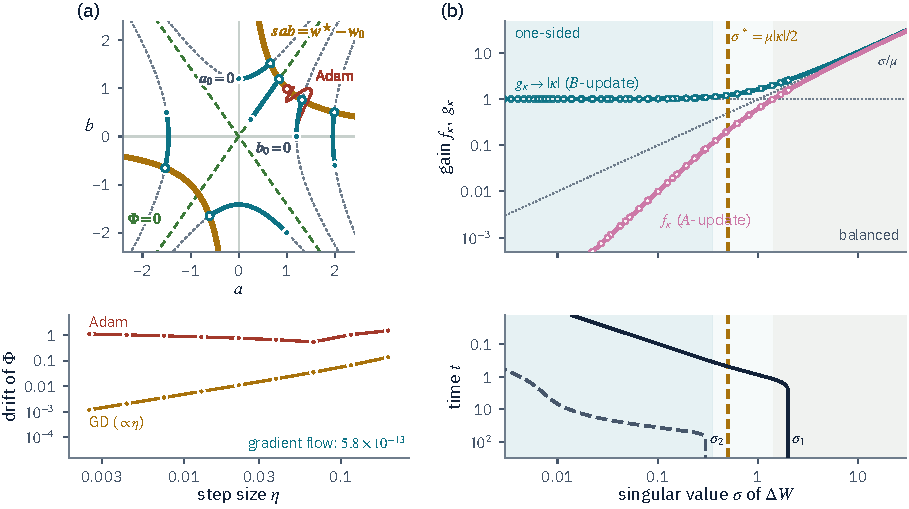
\includegraphics[width=\linewidth]{figures/noether}
\caption{\textbf{Noether hyperbolas and the crossover} (\thmref{Theorem}{III.5}, \thmref{Corollary}{III.6}, \thmref{Theorem}{III.9}). (a)~Scalar LoRA, $w=w_0+s\,ba$ with $s=1$, loss $\tfrac12(w-w^\star)^2$, $w^\star-w_0=1$ and rates $\eta_A=1$, $\eta_B=2$. Top: six gradient-flow trajectories (teal) run from the filled dots along their own charge hyperbolas $b^2/\eta_B-a^2/\eta_A=\Phi_0$ (dashed grey; the slice $\Phi=0$ dashed green) to the fibre $s\,ab=w^\star-w_0$ (ochre). From the zero-$B$ start $(1.2,0)$, Adam (red) leaves its hyperbola and lands at another point of the fibre. Bottom: the drift $\max_{t\le10}\lvert\Phi(t)-\Phi_0\rvert$ from the same start against the step size $\eta$ (learning rates $\eta\eta_A$, $\eta\eta_B$). A GD step changes the charge at order $\eta^2$, so over a fixed time the GD drift is proportional to $\eta$ and vanishes in the flow limit. An Adam step changes the charge at first order in $\eta$, and its drift stays of order one at every step size: Adam lies outside \thmref{Theorem}{III.5} (\thmref{Corollary}{III.6}). (b)~Matrix LoRA with $m=n=6$, $r=2$, loss $\tfrac12\lVert W-W^\star\rVert_F^2$, $B_0=0$ and $A_0A_0^\top=I$ exactly, so that $\Phi=-\kappa I$ with $\kappa=1$ and the crossover lies at $\sigma^*=\mu\lvert\kappa\rvert/2=0.5$ (dashed ochre). Top: the closed-form gains $g_\kappa(\sigma^2/\mu^2)$ (teal, the $B$-update) and $f_\kappa(\sigma^2/\mu^2)$ (purple, the $A$-update) of \thmref{Theorem}{III.9}, with the plateau $\lvert\kappa\rvert$ and the balanced asymptote $\sigma/\mu$ dotted. The hollow circles, read off the factors along the integrated flow for both singular directions, lie on the curves. Shading marks the one-sided regime, the crossover, and the balanced regime (grey). Bottom: the singular values $\sigma_1(t)$ and $\sigma_2(t)$ of $\Delta W$, with time running downward on a log scale. $\sigma_1$ crosses $\sigma^*$ and settles in the balanced regime; $\sigma_2$ stays below $\sigma^*$, where the $A$-update supplies only $7\%$ of its growth rate, as in LoRA-FA. Integrators and tolerances are in \S\ref{app:repro-figures}.}\label{fig:noether}
\end{figure}

A conserved charge is fixed at time zero, so it labels initialisations. Weight decay moves it on purpose, and its two conventions move it toward different targets.

\begin{corollary}{III.6}{charge at initialisation; weight decay}
(a) $\Phi_0=B_0^\top B_0/\eta_B-A_0A_0^\top/\eta_A$ is the value of the conserved charge, fixed by the initialisation and the rates. Since $\Ort(r)$ acts on $\Phi$ by conjugation and preserves $\theta$-trajectories (\thmref{Theorem}{III.5}(ii)), only the spectrum of $\Phi_0$ labels a $\theta$-trajectory.

\smallskip
{\upshape\small\renewcommand{\arraystretch}{1.12}\noindent
\begin{tabularx}{\linewidth}{@{}>{\raggedright\arraybackslash}p{0.5\linewidth}>{\raggedright\arraybackslash}X@{}}
\toprule\headrow
\textbf{Initialisation} & \textbf{Charge $\Phi_0$}\\
\midrule
HF default LoRA on Linear and Conv layers ($B_0=0$; Kaiming-uniform $A_0$ with entries $U(-n^{-1/2},n^{-1/2})$, $n$ the fan-in, which is \texttt{in\_channels} times the kernel size for Conv) & $-A_0A_0^\top/\eta_A$, with $\mathbb{E}[A_0A_0^\top]=\tfrac13I_r$ and fluctuations $O(n^{-1/2})$ on and off the diagonal\\
HF default LoRA on embedding layers ($A_0=0$, normal $B_0$) & $+B_0^\top B_0/\eta_B$ (Init[B]-type)\\
HF \texttt{mica} \citep{rudiger2026mica} ($A_0=0$, frozen minor-singular $B_0$) & $+B_0^\top B_0/\eta_B$ (Init[B]-type, with $B$ frozen)\\
EVA \citep{paischer2024parameter} (orthonormal rows; default \texttt{whiten=False}) & $-I/\eta_A$ exactly\\
PiSSA in HF PEFT \citep{meng2024pissa}, and MiLoRA \citep{wang2024milora} if implemented like \texttt{pissa\_init} with the bottom-$r$ singular values (MiLoRA is not in HF PEFT); $B_0^\top B_0=A_0A_0^\top=S_r/s$, with $S_r$ the top-$r$, resp.\ bottom-$r$, singular values and $s$ the LoRA scale & $(S_r/s)(1/\eta_B-1/\eta_A)$, zero \textbf{iff} $\eta_A=\eta_B$ (when $S_r\ne0$)\\
OLoRA \citep{buyukakyuz2024olora} ($B_0=Q_r$, $A_0=R_r$) & $I/\eta_B-R_rR_r^\top/\eta_A$\\
``Init[B]'' \citep{hayou2024impact} ($A_0=0$) & $+B_0^\top B_0/\eta_B$\\
\bottomrule
\end{tabularx}}
\smallskip

(b) Let $G$ be any cotangent signal, with the scale $s$ absorbed into it. Under gradient flow, if decay acts per unit time and identically on both factors,
\[\dot B=-\eta_BGA^\top-\lambda B,\qquad\dot A=-\eta_AB^\top G-\lambda A,\]
then $\dot\Phi=-2\lambda\Phi$. With learning-rate-coupled decay (PyTorch SGD \texttt{weight\_decay}; the decay term of PyTorch AdamW), $\dot B=-\eta_B(GA^\top+\lambda B)$ and likewise for $A$, so that $\dot\Phi=-2\lambda(B^\top B-AA^\top)$. Then $\Phi(t)=e^{-2\eta\lambda t}\Phi(0)$ holds when $\eta_A=\eta_B=\eta$. For $\eta_A\ne\eta_B$ it fails in general, since $-2\lambda(B^\top B-AA^\top)$ is not a function of $\Phi$. With an actual Adam(W) gradient term, $\Phi$ drifts even without decay, at first order in the step size; Adam lies outside \thmref{Theorem}{III.5}. So neither law describes AdamW training.
\end{corollary}

\noindent\labelsf{Num}\enspace Testing $\Phi(t)=e^{-2\eta_A\lambda t}\Phi(0)$ at $\eta_B/\eta_A=4$ with coupled decay gives a relative error of $10.7$; in the valid cases the error is that of the integrator, between $10^{-8}$ and $2\times10^{-4}$. One Adam sign step moves $\Phi$ by an amount proportional to the learning rate, while an SGD step moves $\eta\Phi$ at second order (Appendix~\ref{app:repro}).

\begin{explains}
\begin{itemize}
\item Zero-product initialisations keep their charge under gradient flow, and that charge is maximally unbalanced (\thmref{Proposition}{III.8}). The \emph{relative} imbalance $\|\Phi\|/(\|B\|^2/\eta_B+\|A\|^2/\eta_A)$ decays as the adapter grows (\thmref{Theorem}{III.9}).
\item HF PiSSA always has $\mu_0=B_0^\top B_0-A_0A_0^\top=0$ (unweighted-balanced), and $\Phi_0=0$ only at equal rates. So it starts on the slice that coupled decay targets, and off the per-time-decay slice when $\eta_A\ne\eta_B$.
\item Both decay conventions gauge-fix at equilibrium, because each is a $\Lambda$-gradient flow of $L$ plus a fibre-wise Kempf--Ness potential (\bgref{D.30}). Per-time decay is the flow of $L+\tfrac\lambda2(\|B\|^2/\eta_B+\|A\|^2/\eta_A)$; it drives $\Phi\to0$ exponentially, onto the rate-weighted slice $B^\top B/\eta_B=AA^\top/\eta_A$. Coupled decay is the flow of $L+\tfrac\lambda2(\|B\|^2+\|A\|^2)$; its equilibria lie on the unweighted balanced slice $\mu=B^\top B-AA^\top=0$ of \thmref{Proposition}{III.7}(a), with no closed-form law for $\Phi$ unless $\eta_A=\eta_B$. The two slices coincide iff $\eta_A=\eta_B$. In particular, coupled decay also gauge-fixes at LoRA+ rates, onto $\mu=0$.
\end{itemize}
\end{explains}

\noindent\labelsf{Num}\enspace At $\eta_B/\eta_A=4$, coupled decay converges to $\mu=0$ to within $10^{-12}$ while $\Phi$ stays of order $1$; per-time decay converges to $\Phi=0$ while $\mu$ stays of order $1$ (Appendix~\ref{app:repro}).

The names Init[A] and Init[B], and the finding that these zero-product starts train differently, are due to \citet{hayou2024impact}. Exponential decay of such charges under weight decay is the rescale-symmetry law of \citet{kunin2020neural}.

\subsubsection{The balanced slice}\label{sec:fibres-balance}

In Kempf--Ness theory, the least-norm vectors on a closed orbit of a reductive group form one orbit of its compact part, and they are where the moment map vanishes (\bgref{D.29}, \bgref{D.30}). For LoRA the moment map is $\mu=B^\top B-AA^\top$, and the least-norm representatives are the balanced ones.

\begin{proposition}{III.7}{Kempf--Ness slice; Loewner floor; known, \citet{xkempf1979length,xsrebro2004maximum}}
(a) On a full-rank $\GL_r$-orbit, the critical points of $\|B\|^2+\|A\|^2$ are exactly the balanced representatives, those with $\mu=B^\top B-AA^\top=0$. They form one $\Ort(r)$-orbit, they are the minima, and the minimum value is $2\|BA\|_*$.

(b) Assume gradient flow with block-scalar rates $\eta_A,\eta_B$, no weight decay, a loss that depends on $(B,A)$ only through $BA$, and any cotangent signal of the form $\Lambda D\rho^\top\gamma$ (dropout, minibatches and clipping included). From $B_0=0$,
\[B^\top B=\tfrac{\eta_B}{\eta_A}\big(AA^\top-A_0A_0^\top\big)\succeq0,\]
so $AA^\top\succeq A_0A_0^\top$ for all time; the $A$-factor never shrinks below its initialisation in the Loewner order. $AA^\top(t)$ need not be monotone in $t$; only this floor is guaranteed. Discrete steps break the bound by $O(\eta^2)$ per step. Under Adam it is not guaranteed and fails empirically. With per-time decay $\lambda$, only $AA^\top\succeq e^{-2\lambda t}A_0A_0^\top$ holds.
\end{proposition}

Part (a) is the theorem of \citet{xkempf1979length}, in the real form of \citet{xrichardson1990minimum}; the nuclear-norm identity is due to \citet{xsrebro2004maximum}. BaLoRA \citep{castin2026balanced} turns the slice into an algorithm, moving after every step to a product-preserving representative with $B^\top B=AA^\top$ diagonal.

\noindent\labelsf{Num}\enspace On $5$ random orbits at $(m,n,r)=(7,5,3)$ the minimum equals $2\|BA\|_*$ to within $10^{-14}$ (Appendix~\ref{app:repro}).

\begin{explains}
Balancedness is a precise notion: it is the Kempf--Ness slice of the gauge action. An explicit penalty $\lambda(\|B\|^2+\|A\|^2)$ is equivalent at its minimisers to a $(2\lambda/s)$-nuclear-norm penalty on $\Delta W=sBA$ restricted to rank $\le r$. SGD-coupled decay with coefficient $\lambda$ is the flow of $L+\tfrac\lambda2(\|B\|^2+\|A\|^2)$ and matches a $(\lambda/s)$-nuclear-norm penalty (\citealp{xsrebro2004maximum}, whose argument also covers rank-deficient factorisations). In both cases the stationary points lie on $\mu=0$. With per-time decay at unequal rates the relevant slice is $\Phi=0$ (\thmref{Corollary}{III.6}). Decoupled AdamW decay is not covered.
\end{explains}

The default start is as unbalanced as possible, and no start meets all three natural wishes.

\begin{proposition}{III.8}{the balance--escape trilemma}
No LoRA initialisation is simultaneously
\begin{enumerate}[label=(\alph*)]
\item identity-at-init without a residual split ($B_0A_0=0$),
\item balanced ($B_0^\top B_0=cA_0A_0^\top$ for some $c>0$: unweighted, $c=1$, or rate-weighted, $\Phi_0=0$ with $c=\eta_B/\eta_A$), and
\item non-stationary, meaning that $D\rho$ at $(B_0,A_0)$ is not the zero map; equivalently, $\dot W(0)\ne0$ for some parameter velocity, under any first-order optimizer.
\end{enumerate}
Moreover, if $B_0A_0=0$ then $\langle B_0^\top B_0,A_0A_0^\top\rangle_F=0$, so
\[\|B_0^\top B_0-cA_0A_0^\top\|_F^2=\|B_0^\top B_0\|_F^2+c^2\|A_0A_0^\top\|_F^2,\]
and zero-product initialisations are maximally unbalanced.
\end{proposition}

\begin{explains}
The field splits into two families of initialisation.
\begin{itemize}
\item \textbf{Type I} keeps $\rho$ and picks $q_0$ in the apex fibre $\{BA=0\}$: LoRA, EVA, Init[B]. By the identity above these are maximally unbalanced.
\item \textbf{Type II} changes $\rho$ by an exact split $\theta_0=\theta_{\mathrm{res}}+\delta(q_0)$: PiSSA, MiLoRA, OLoRA, LoRA-GA \citep{wang2024lorab}, CorDA \citep{yang2024corda}. LoftQ \citep{li2023loftq} and QPiSSA \citep{meng2024pissa} are approximate splits over a quantised residual, so they are not identity-at-init (\thmref{Proposition}{V.2}).
\end{itemize}
The proposition forces every balanced, non-stationary, identity-at-init LoRA initialisation to be Type II. The converse fails: OLoRA ($B_0^\top B_0=I$, $A_0A_0^\top=R_rR_r^\top$) and CorDA are Type II and generally unbalanced. A frozen residual is the price of any nonzero $B_0A_0$, and so in particular of balance, as in PiSSA and MiLoRA at equal rates. By \thmref{Theorem}{II.2}, Type II objects are different objects, incomparable with LoRA.
\end{explains}
